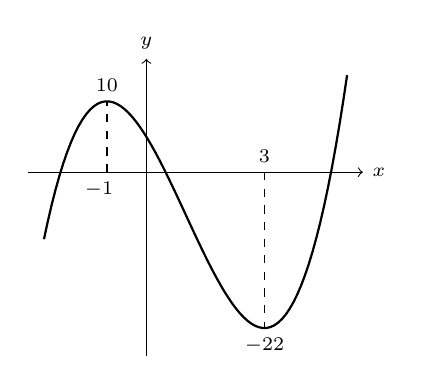
\begin{tikzpicture}[x=5mm,y=0.9mm]
\draw[->] (-3,0)--(5.5,0) node[right]{\scriptsize $x$};
\draw[->] (0,-26)--(0,16) node[above]{\scriptsize $y$};
\draw[thick,domain=-2.6:5.1,samples=80] plot (\x,{\x*\x*\x-3*\x*\x-9*\x+5});
\draw[dashed] (-1,0)--(-1,10) (3,0)--(3,-22);
\node[above] at (-1,10){\scriptsize 10}; \node[below] at (3,-22){\scriptsize $-22$};
\node[below] at (-1.2,0){\scriptsize $-1$}; \node[above] at (3,0){\scriptsize 3};
\end{tikzpicture}